\documentclass[10pt,a4paper]{article}
\usepackage{rpgcover} % Loads the original rpgmanual.sty and its fonts
\babelprovide[import]{french}
\usepackage{xsavebox}
\RPGSetRunningTitle{Le sentier des dettes}
\hypersetup{pdftitle={Le sentier des dettes — Au dernier lancer},pdfauthor={Jacopo Biscella}}
\RPGSetCoverWordSpace{.78em}
% Paragraph spacing and leading of the French adventure and manual-fr.tex.
\setlength{\parskip}{2pt plus .5pt minus .5pt}
\linespread{1.025}\selectfont
% JPEG copies of the shared cover backgrounds (scripts/build-adventure-print-art.sh), as in the adventure.
\RPGSetFrontBackground{assets/engraved-front-background.jpg}\RPGSetBackBackground{assets/engraved-cover-background.jpg}
% The adventure's front-cover typography, with the overlay saved once (xsavebox) and reused on the
% contents page instead of being embedded twice.
\newcommand{\SentieroFrontCover}{%
 \clearpage\RPGCoverPagetrue\thispagestyle{empty}\null
 \xsavebox{SentieroOverlay}{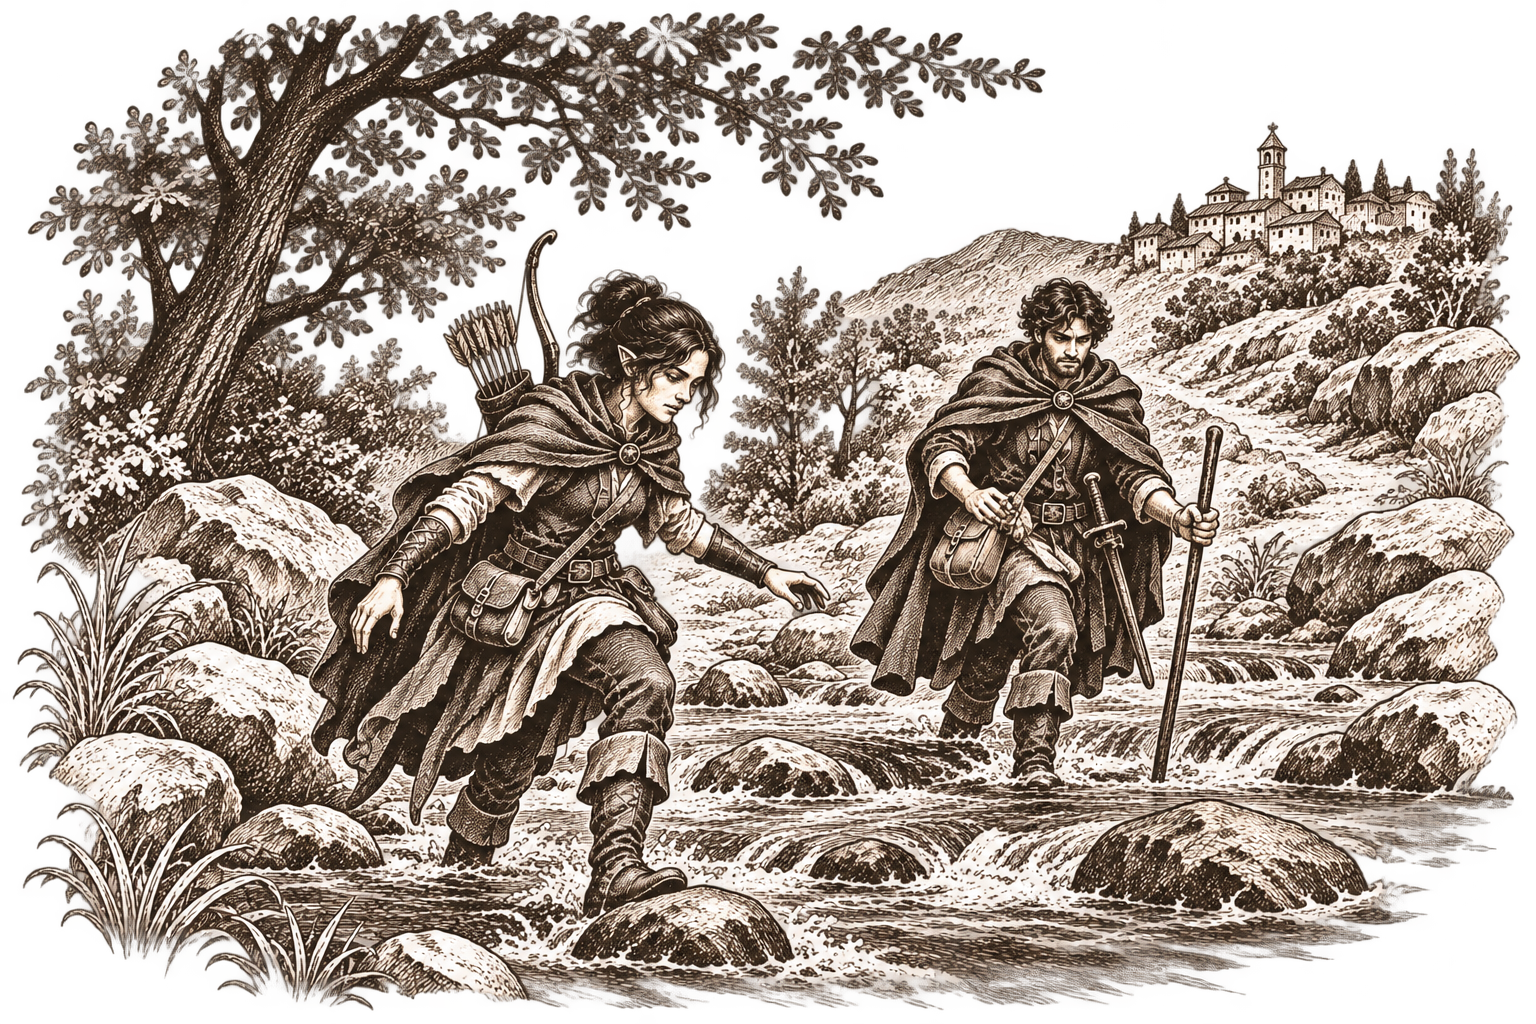
\includegraphics{assets/path-of-debts/front-overlay.png}}%
 \begin{tikzpicture}[remember picture,overlay,x=1mm,y=1mm]
  \RPGDrawBackground{\RPGFrontBackgroundFile}
  % Title and subtitle as on the adventure's cover: same sizes and positions in the cartouche.
  \node[align=center,text=coverink,text width=138mm,inner sep=0pt] at ($(current page.south west)+(105mm,248mm)$)
   {\RPGCoverTitleFont\fontsize{16.6}{20.7}\selectfont\spaceskip=\RPGCoverWordSpace\relax LE SENTIER\\[1.0mm]DES DETTES};
  \node[align=center,text=coverink,text width=135mm,inner sep=0pt] at ($(current page.south west)+(105mm,235mm)$)
   {\RPGCoverSubtitleFont\fontsize{9.5}{12}\selectfont Un récit d’introduction pour «~Au dernier lancer~»};
  \node[inner sep=0pt,anchor=center] at ($(current page.south west)+(105mm,125mm)$)
   {\resizebox{150mm}{!}{\xusebox{SentieroOverlay}}};
  \node[align=center,text=coverink,text width=124mm,inner sep=0pt] at ($(current page.south west)+(105mm,25mm)$)
   {\RPGCoverTextFont\fontsize{12}{15}\selectfont Jacopo Biscella};
 \end{tikzpicture}
 \clearpage\RPGCoverPagefalse}
% Uses precisely the back background and the editable cover fonts from rpgcover.sty.
% This is text layout only: no substitute illustrations or background graphics.
\newcommand{\SentieroBackCover}{%
 \clearpage\pagenumbering{gobble}\RPGCoverPagetrue\thispagestyle{empty}\null
 \begin{tikzpicture}[remember picture,overlay,x=1mm,y=1mm]
   \RPGDrawBackground{\RPGBackBackgroundFile}
   \node[align=center,text=coverink,text width=170mm,inner sep=0pt]
     at ($(current page.south west)+(105mm,260mm)$)
     {{\RPGCoverTitleFont\fontsize{19}{23}\selectfont\spaceskip=\RPGCoverWordSpace\relax LE SENTIER DES DETTES}};
   \draw[coverink,line width=.45pt]
     ($(current page.south west)+(57mm,246mm)$)--($(current page.south west)+(153mm,246mm)$);
   % Blocks at the positions of the adventure's back cover: story at 240 mm, small-caps lines at
   % 197, second rule at 167, description at 162, closing line at 133.
   \node[anchor=north,align=left,text=coverink,text width=137mm,inner sep=0pt]
     at ($(current page.south west)+(105mm,240mm)$)
     {\RPGCoverTextFont\fontsize{10.4}{13.4}\selectfont
      Une fausse pièce. Une lettre sans destinataire. Deux voyageurs sans aucune raison de se faire confiance.\par\smallskip
      Nim Thistledown et Mara Veyne suivent la route du roi jusqu’à l’Âtre Creux. En chemin, ils apprendront qu’une promesse peut être plus dangereuse qu’une arme, et que certains choix ont des conséquences même quand personne ne les voit.};
   \node[anchor=north,align=center,text=coverink,text width=140mm,inner sep=0pt]
     at ($(current page.south west)+(105mm,197mm)$)
     {\RPGCoverSubtitleFont\fontsize{13}{17}\selectfont
      Un prologue à «~La cloche de l’Âtre Creux~»};
   \draw[coverink,line width=.45pt]
     ($(current page.south west)+(57mm,167mm)$)--($(current page.south west)+(153mm,167mm)$);
   \node[anchor=north,align=left,text=coverink,text width=137mm,inner sep=0pt]
     at ($(current page.south west)+(105mm,162mm)$)
     {\RPGCoverTextFont\fontsize{10.4}{13.4}\selectfont
      Sept exemples montrent comment les décisions des joueurs deviennent des jets, des dialogues et des conséquences à la table d’Au dernier lancer.};
   \node[anchor=north,align=center,text=coverink,text width=147mm,inner sep=0pt]
     at ($(current page.south west)+(105mm,133mm)$)
     {\RPGCoverSubtitleFont\fontsize{10.5}{13.2}\selectfont
      Le récit s’achève là où commence l’aventure.};
   \filldraw[fill=white,draw=coverink,line width=.55pt]
     ($(current page.south west)+(139mm,25mm)$) rectangle
     ($(current page.south west)+(187mm,55mm)$);
 \end{tikzpicture}
 \clearpage\RPGCoverPagefalse
}
% Dice icons for the "À la table" boxes, drawn with TikZ (no font glyphs, so they work in every
% language). \Dado{n}: a kept d6 showing n; \Dado*{n}: a rolled die that is not kept (faded).
% \Su and \Giu: the rulebook's keep-highest and keep-lowest arrows, from FreeSerif.
% \Bersaglio: the TN to reach. \Riuscita and \Fallita: success and failure.
\newcommand\DadoPips[1]{%
  \ifcase#1\or \fill (.5,.5) circle (.1);
  \or \fill (.27,.73) circle (.1); \fill (.73,.27) circle (.1);
  \or \fill (.25,.75) circle (.09); \fill (.5,.5) circle (.09); \fill (.75,.25) circle (.09);
  \or \foreach \x/\y in {.27/.27,.27/.73,.73/.27,.73/.73}{\fill (\x,\y) circle (.095);}
  \or \foreach \x/\y in {.25/.25,.25/.75,.75/.25,.75/.75,.5/.5}{\fill (\x,\y) circle (.09);}
  \or \foreach \x/\y in {.28/.22,.28/.5,.28/.78,.72/.22,.72/.5,.72/.78}{\fill (\x,\y) circle (.085);}
  \fi}
\makeatletter
% A die that is set aside has a dashed outline and lighter pips, but stays legible.
\tikzset{dado kept/.style={draw=rpgbrown,fill=white},dado dropped/.style={draw=rpgbrown,fill=rpgshade,dash pattern=on .9pt off .6pt},
  pips kept/.style={fill=rpgink},pips dropped/.style={fill=rpgbrown!70}}
\newcommand\Dado{\@ifstar{\Dado@{dropped}}{\Dado@{kept}}}
\newcommand\Dado@[2]{\tikz[baseline=-.1em,x=.95em,y=.95em]{%
  \path[dado #1,line width=.5pt,rounded corners=1.2pt] (0,-.12) rectangle (1,.88);
  \begin{scope}[shift={(0,-.12)},pips #1]\DadoPips{#2}\end{scope}}}
\makeatother
\newcommand\Su{{\fontspec{FreeSerif}↑}}
\newcommand\Giu{{\fontspec{FreeSerif}↓}}
\newcommand\Riuscita{\tikz[baseline=-.1em,x=1em,y=1em]{\draw[rpgbrown,line width=1.1pt,line cap=round,line join=round] (.08,.35)--(.38,.05)--(.92,.75);}}
\newcommand\Fallita{\tikz[baseline=-.1em,x=1em,y=1em]{\draw[rpgbrown,line width=1.1pt,line cap=round] (.15,.05)--(.85,.75) (.15,.75)--(.85,.05);}}
\newcommand\Bersaglio{\tikz[baseline=-.1em,x=1em,y=1em]{\draw[rpgbrown,line width=.6pt] (.5,.38) circle (.45) (.5,.38) circle (.25); \fill[rpgbrown] (.5,.38) circle (.08);}}
\begin{document}
% Select the language here: babel resets to its main language (english) at \begin{document}.
\selectlanguage{french}
\RPGStartFrontMatter
\SentieroFrontCover
\RPGStartContents
\clearpage\thispagestyle{rpgfrontmatter}
\vspace*{9mm}
\begin{center}{\fontsize{27}{31}\selectfont\bfseries SOMMAIRE\par}\vspace{9pt}
{\color{rpgline}\rule{.76\linewidth}{.55pt}}\end{center}\vspace{8mm}
\begingroup
\makeatletter
\renewcommand{\l@section}[2]{\@dottedtocline{1}{0em}{4em}{\bfseries #1}{#2}}
\@starttoc{toc}
\makeatother
\endgroup
\vfill
\begin{center}\resizebox{.58\linewidth}{!}{\xusebox{SentieroOverlay}}\end{center}
\vfill
\begin{center}{\small\itshape Un récit d’introduction pour Au dernier lancer\par}
\vspace{4pt}{\footnotesize Jacopo Biscella\par}\vspace{5pt}
{\footnotesize Ce récit est diffusé sous licence Creative Commons Attribution — Partage dans les mêmes conditions 4.0 International (CC BY-SA 4.0), comme Au dernier lancer. Vous pouvez le partager et l’adapter, y compris commercialement, en créditant l’auteur et en conservant la même licence.\par}\end{center}
\clearpage
\RPGStartMainMatter
\RPGChapter{Une mauvaise pièce}
La pièce avait une tête de chaque côté. L’une portait la couronne du roi~; l’autre, le visage d’un homme que le roi avait fait pendre vingt ans plus tôt.

L’érudit Mara Veyne la fit tourner entre le pouce et l’index. Le cuivre n’était usé que d’un côté. Celui qui l’avait frappée voulait que la ruse dure peu~: assez pour changer de mains, pas assez pour tomber sous les yeux d’un percepteur.

«~Je t’ai dit qu’elle était fausse~», dit le marchand.

«~Je n’ai pas dit le contraire.~»

«~Alors pourquoi tu la regardes depuis une demi-heure~?~»

«~Pour comprendre qui veut s’en servir.~»

Ils étaient assis à une table du relais de poste des Trois Gués. Il pleuvait depuis quatre jours. La route du roi n’était plus qu’une longue bande de boue où charrettes et chevaux avançaient à grand-peine. Le marchand avait vendu à Mara une place sur le chariot pour le tronçon vers le nord, avec une promesse~: il pourrait consulter le registre des marchandises avant d’arriver au carrefour.

Cette promesse, Mara l’avait compris, valait plus que le voyage.

Le registre énumérait les villages que desservait le chariot. Parmi eux, d’une autre écriture, figurait \textbf{l’Âtre Creux}. À côté du nom, quelqu’un avait tracé une marque ronde, puis l’avait rayée.

«~Cet endroit n’est plus sur ma tournée~», dit le marchand en voyant où il regardait.

«~Depuis quand~?~»

«~Depuis que le prix du bois ne couvre plus le coût du voyage.~»

«~Et cette marque~?~»

L’homme referma le registre. «~Une bricole, pour suivre une livraison. Le chariot part à l’aube. Tu viens toujours~?~»

Mara posa la pièce sur la table, côté roi visible. «~Oui.~»

Il ne dit pas au marchand qu’il avait vu une écriture semblable des années plus tôt, dans la marge d’un vieux registre. Il ne lui demanda pas non plus pourquoi quelqu’un avait gratté une date pour en écrire une autre. Il avait appris que les questions posées trop tôt rendent prudents même les menteurs les plus maladroits.

Cette nuit-là, il recopia le nom du village à la fin de ses notes. Puis il changea d’itinéraire. Le chariot irait vers le nord. Mara, au carrefour, prendrait le sentier de la forêt.
\begin{rpgnote}
\textbf{Comment lire les encadrés.} Dans les encadrés \emph{À la table}, les dés sont dessinés~: \Dado{5}~dé gardé, \Dado*{2}~dé écarté, \Bersaglio~SD à atteindre, \Riuscita~réussite, \Fallita~échec. Les niveaux s’écrivent comme sur la fiche~: Novice 2d6\Giu\ (garder le plus faible), Compétent 1d6, Expert 2d6\Su\ (garder le plus élevé), Exceptionnel 3d6\Su. Le SD est le Seuil de difficulté, la valeur à atteindre. Proche est l’une des distances du manuel~: quelques pas, accès immédiat.
\end{rpgnote}
\begin{rpgexample}{À la table · Le premier jet}
\textbf{Narrateur~:} «~Le marchand referme le registre. Mara a vu le nom du village et une date grattée. À première vue, la date est illisible. Comment essaies-tu de la déchiffrer~?~»

\textbf{Joueur de Mara~:} «~Je compare les traces des chiffres avec les autres dates de la même écriture. Je n’utilise pas Histoire~: je n’ai pas besoin de me rappeler ce qui s’est passé, j’ai besoin de lire des marques effacées.~»

\textbf{Narrateur~:} «~Alors c’est du Savoir, \Bersaglio\,SD~4. Mara est Expert~: lance 2d6\Su, deux dés, et garde le plus élevé.~»

\textbf{Joueur de Mara~:} «~J’obtiens \Dado*{2}\,\Dado{5}~: je garde 5.~» \Riuscita

\textbf{Narrateur~:} «~Tu réussis. La date remonte à deux semaines, pas à hier. Le nom du village, en revanche, tu le connaissais déjà~: il n’a jamais dépendu du jet.~»

\emph{On fait un jet quand l’issue est incertaine. Le niveau Expert lance 2d6 et garde le meilleur dé~: 5 atteint le SD~4. Un indice essentiel n’est jamais caché derrière un jet.}

\end{rpgexample}
\RPGChapter{La troisième route}
Nim Thistledown ne prit pas la bourse tout de suite.

Le charretier la tenait ouverte, avec l’air de quelqu’un qui attend des remerciements. Dedans, il y avait six pièces d’argent et une feuille de papier pliée en quatre.

«~Le paiement convenu~», dit-il.

«~Pour la route que nous connaissons tous les deux, peut-être.~»

«~Pour une livraison.~»

«~Alors pourquoi ne la fais-tu pas toi-même~?~»

Le charretier montra son chariot, arrêté devant l’écurie avec une roue cassée. «~Parce qu’il me manque un cheval, une roue et l’envie de me faire tuer pour une lettre.~»

Nim déplia le papier. Il n’était pas cacheté. Il contenait deux lignes~: \emph{La moitié de la dette est payée. L’autre moitié, en argent du Nord, quand la cloche se taira.} En bas figurait le nom d’une auberge de l’Âtre Creux, mais pas celui du destinataire.

«~Qui t’a donné ça~?~»

«~Un homme au carrefour. Manteau gris, capuchon relevé. Il disait les bons mots, mais en appuyant sur les mauvaises syllabes, comme quelqu’un qui les a appris à l’oreille.~»

Nim replia la feuille. «~Et son nom~?~»

«~Il ne me l’a pas donné. Il m’a donné de l’argent. Tu prends ou tu laisses~?~»

Nim prit la bourse, mais compta les pièces une à une. La sixième était mince, presque lisse. «~Il en manque deux.~»

Le charretier soupira et ajouta une pièce. Nim s’éloigna avant qu’il ne change d’avis.

Elle n’avait aucune intention de livrer la lettre à l’aveugle. C’était assez d’argent pour trois jours de route~; trop pour un message sans nom. Et une cloche qui devait se taire n’était pas une phrase à livrer sans la comprendre.

La troisième route partait derrière les écuries, là où la boue gardait peu d’empreintes. Un chemin rapide, d’après la carte~; un chemin abandonné, d’après les gens du coin. Nim se mit en route en comptant ses pas jusqu’au premier embranchement.
\RPGChapter{L’arbre tombé}
Mara rencontra Nim après midi, devant un tronc qui barrait le sentier.

Nim examinait le sol. Elle avait posé son sac sur une pierre et tenait une brindille entre les dents.

«~La forêt est fermée~?~» demanda Mara.

«~Ça dépend à quel point tu aimes les raccourcis.~»

«~Pas beaucoup.~»

«~Alors nous avons quelque chose en commun.~»

Le tronc d’un hêtre gisait en travers du chemin, les racines encore enfoncées dans la terre. Il était tombé récemment. Les feuilles étaient vertes, l’écorce humide. Il n’y avait pas eu de vent assez fort pour l’abattre.

Mara s’accroupit pour examiner un éclat de bois. Une sève claire suintait de l’entaille.

«~Une hache~», dit-il.

«~Deux, répondit Nim. Quelqu’un a travaillé de ce côté, et un autre de l’autre côté.~»

Mara regarda les entailles~: parallèles, régulières, trop basses pour quelqu’un qui cherchait du bois de chauffage. «~Ils l’ont abattu uniquement pour fermer le chemin.~»

«~Il y a des empreintes qui repartent en arrière. De l’autre côté, aucune.~»

«~Tu sais lire les empreintes~?~»

«~Je sais voir où quelqu’un a essayé de les effacer.~»

Mara eut un léger sourire. Nim se glissa sous le tronc, en ressortit la manche couverte de boue et montra une étroite ouverture entre les racines. «~On peut passer, mais ceux qui ont un chariot devront faire demi-tour.~»

«~Et ceux qui ont des livres~?~»

«~Ça dépend combien.~»

Mara tapota sa sacoche. «~Trop.~»

Ils n’échangèrent leurs noms qu’une fois l’obstacle franchi. Ce n’était pas une grande preuve de confiance. Mais Mara cessa de garder une main sur le fermoir de sa sacoche chaque fois que Nim s’approchait.
\RPGChapter{L’éboulement}
Ils trouvèrent l’éboulement près d’une heure plus tard.

Le sentier longeait le flanc de la colline, au-dessus d’un torrent gonflé. Sur une vingtaine de pas, il n’existait plus~: la pluie avait arraché une bande de pente, et à sa place une langue de boue et de pierres descendait jusqu’à l’eau. De temps en temps, une pierre se détachait et roulait en bas sans se presser. Quelqu’un était passé la veille~: les empreintes allaient jusqu’à mi-chemin et disparaissaient sous un glissement plus récent.

Nim étudia la pente. «~Nous pourrions remonter jusqu’au gué.~»

«~Combien de temps faudrait-il~?~»

«~Deux heures, peut-être trois.~»

Mara leva les yeux. Les nuages recommençaient à cacher le soleil. «~Et jusqu’au village~?~»

«~Encore une demi-journée.~»

«~Alors nous arriverions de nuit.~»

Nim regarda l’éboulement. Là où la boue avait mis la roche à nu, un pied pouvait trouver prise~; ailleurs, la terre cédait au moindre contact. «~Si je traverse vite et léger, la pente n’aura pas le temps de bouger.~»

«~Tu pourrais aussi tomber.~»

«~C’est une des possibilités.~»

Mara serra sur sa poitrine la sangle de sa sacoche. «~Alors tu ne traverses pas seule. Je passe derrière toi, je mets les pieds où tu mets les tiens et je te tiens par la ceinture. Si tu glisses, je te retiens.~»

«~Et si c’est toi qui glisses, tu m’entraînes avec toi.~»

«~Alors essaie de ne pas me faire glisser.~»

Nim le regarda un instant. Puis elle se tourna vers l’éboulement et s’élança. Mara la suivit, une main serrée sur sa ceinture.

À mi-chemin, une motte céda sous le pied de Nim. La boue bougea d’un seul bloc, comme une couverture tirée d’un côté. Nim bascula en avant~; Mara cala ses talons contre une pierre et tira. La ceinture tint. Un instant, ils restèrent immobiles, tandis que les pierres délogées roulaient jusqu’au torrent.

Puis Nim trouva la roche, et Mara la suivit pas à pas.

Quand ils atteignirent l’autre côté, Mara avait les jambes qui tremblaient. Nim se retourna~: le passage avait déjà disparu sous une nouvelle couche de boue.

«~Deux heures de gagnées~», dit-elle.

«~Tu n’as pas compté les dix ans de vie que je viens de perdre.~»

«~Ils n’étaient pas sur la carte.~»
\begin{rpgexample}{À la table · Traverser et aider}
\textbf{Narrateur~:} «~L’éboulement bouge encore. Le traverser, c’est de la Dextérité, \Bersaglio\,SD~4. Si tu échoues, tu glisses vers le torrent.~»

\textbf{Joueuse de Nim~:} «~Nim est Experte en Dextérité~: 2d6\Su. Mara peut m’aider~?~»

\textbf{Joueur de Mara~:} «~Je marche juste derrière elle et je la tiens par la ceinture. Si elle glisse, je la retiens.~»

\textbf{Narrateur~:} «~Vous traversez ensemble et c’est celle qui ouvre la marche qui lance~: Nim. Mara est Novice en Dextérité et n’a aucune Compétence qui l’aide~: pour le même test, il ne lancerait pas au niveau Expert, donc son aide est une Aide incompétente. Elle ajoute un dé au jet de Nim, mais le SD passe de 4 à 5~: à deux sur la boue, vous délogez plus de pierres. Vous acceptez~?~»

\textbf{Joueuse de Nim~:} «~Oui. Si je glisse seule, je n’ai rien à quoi me retenir.~»

\textbf{Narrateur~:} «~Alors Nim lance 3d6\Su\ contre \Bersaglio\,SD~5.~»

\textbf{Joueuse de Nim~:} «~J’obtiens \Dado*{1}\,\Dado*{4}\,\Dado{5}~: je garde 5.~» \Riuscita

\textbf{Narrateur~:} «~Vous êtes passés. À mi-chemin, une motte cède sous Nim, et Mara la retient par la ceinture. De l’autre côté, vous vous retournez~: le passage a déjà disparu sous la boue. Aucun chariot ne passera par ici.~»

\emph{Une Aide incompétente ajoute 1d6 mais augmente le SD de 1. Avec 1, 4 et 5, Nim atteint le nouveau SD~5. La main de Mara sur la ceinture est la façon dont l’Aide entre dans l’histoire~: elle ne remplace pas le jet.}

\end{rpgexample}
\RPGChapter{Deux personnes sur la route}
Ils marchèrent jusqu’à ce que le sentier devienne aussi large qu’une route. Ils virent alors le chariot.

Il avait de hautes roues, un plateau couvert d’une toile cirée et un cheval gris qui mangeait les feuilles les plus basses d’un noisetier. Le conducteur dormait sur le banc, le chapeau sur le visage. Une femme était penchée sur le moyeu de la roue droite.

«~Pouvons-nous aider~?~» demanda Mara.

La femme se redressa. Elle avait les mains noires de graisse et un couteau de travail pendu à la ceinture. «~Si vous avez une goupille de rechange.~»

Nim regarda la roue. «~Pas besoin de la changer. C’est le crochet qui est tordu.~»

«~Et comment tu le sais~?~»

«~Parce que la goupille est toujours en place.~»

La femme lui tendit le marteau sans un mot. Nim s’accroupit, fit levier avec une pierre plate et frappa trois coups précis. Le crochet redevint presque droit.

«~Essaie maintenant~», dit-elle.

La femme tira sur la roue. Elle tournait.

Le conducteur se réveilla au bruit. Il demanda qui ils étaient, pourquoi ils touchaient au chariot et s’ils essayaient de le voler. La femme lui dit de se taire.

«~Vous allez à l’Âtre Creux~?~» demanda Mara.

La femme cessa de s’essuyer les mains. «~Nous y passions, jusqu’à il y a peu.~»

«~Et maintenant~?~»

«~Maintenant, nous préférons perdre une journée.~»

Elle ne voulut pas en dire plus, mais leur donna un morceau de pain et un fromage dur enveloppé dans une feuille. Quand le conducteur eut le dos tourné, elle parla à voix basse.

«~La route du nord est pleine d’hommes qui réclament des péages sans en avoir le droit. Ils ne portent pas d’uniforme. L’un d’eux en portait un, autrefois.~»

«~Où ça~?~» demanda Nim.

«~Au carrefour des Trois Pierres. Si vous le croisez, ne dites pas que vous m’avez aidée.~»

Mara n’insista pas. Avant de repartir, Nim s’accroupit près des ornières. Parmi les empreintes du cheval, il y en avait d’autres, celles de deux personnes à pied~: elles avaient suivi le chariot presque jusqu’au noisetier, puis étaient reparties vers le nord.

«~Ce n’est pas un avertissement par ouï-dire, dit Nim à la femme. Vous les avez déjà rencontrés.~»

La femme regarda les empreintes et hocha la tête. «~L’un est jeune. L’autre ne se montre pas, s’il peut l’éviter.~»

Elle les laissa partir d’un signe de tête et retourna au chariot.
\begin{rpgexample}{À la table · Quand une Compétence change le jet}
\textbf{Narrateur~:} «~Le crochet est tordu. Nim, comment essaies-tu de le réparer~?~»

\textbf{Joueuse de Nim~:} «~Avec le marteau de la charretière et une pierre pour caler.~»

\textbf{Narrateur~:} «~Une vraie réparation, ce serait du Savoir avec Artisanat. Ici, il suffit de redresser le crochet en trois coups précis~: Dextérité, \Bersaglio\,SD~4. Si tu échoues, tu risques de le casser.~»

\textbf{Joueuse de Nim~:} «~Nim est Experte en Dextérité~: 2d6\Su. Aucune de ses Compétences ne concerne les marteaux, donc pas de degré en plus. J’obtiens \Dado*{3}\,\Dado{5}~: je garde 5.~» \Riuscita

\textbf{Narrateur~:} «~La roue tourne de nouveau. Au moment de repartir, tu remarques des empreintes à côté des ornières. Tu veux les examiner~?~»

\textbf{Joueuse de Nim~:} «~Oui. Nim a Survie, une Compétence de Dextérité faite justement pour suivre des traces.~»

\textbf{Narrateur~:} «~Comprendre qui a suivi le chariot, c’est \Bersaglio\,SD~4. Dextérité Expert plus Survie~: tu montes d’un degré, à Exceptionnel. Lance 3d6\Su.~»

\textbf{Joueuse de Nim~:} «~J’obtiens \Dado*{2}\,\Dado*{4}\,\Dado{6}~: je garde 6.~» \Riuscita

\textbf{Narrateur~:} «~Tu distingues deux séries d’empreintes~: elles ont suivi le chariot, puis ont tourné vers le nord. La femme confirme qu’elle a déjà rencontré les faux péagers.~»

\emph{Les valeurs sont celles de la fiche de Nim~: Experte en Dextérité, avec Survie et sans Artisanat, qui est de toute façon une Compétence de Savoir. Une Compétence pertinente améliore le jet d’un degré. Un seul 6 n’est pas un Critique~: il en faut au moins deux.}

\end{rpgexample}
\RPGChapter{Le carrefour des Trois Pierres}
Au carrefour se dressaient trois bornes, mais deux seulement tenaient encore debout. La troisième gisait sur le flanc, à moitié cachée dans l’herbe. Quelqu’un avait gravé une marque récente dans la mousse~: un cercle barré d’un trait.

Nim y reconnut la marque d’un collecteur d’impôts itinérant. Elle l’avait vue sur des reçus vrais et faux, plus souvent faux que vrais.

«~Le péage est une escroquerie~», dit-elle.

«~Ce n’est pas une surprise.~»

«~Le choix de l’endroit, si. Il n’y a rien ici qui vaille la peine d’être protégé.~»

«~Une route, répondit Mara, est utile même sans rien autour.~»

Un bref silence suivit. Puis une voix s’éleva derrière les buissons.

«~Vingt pièces pour passer.~»

L’homme qui sortit à découvert était jeune. Il portait un manteau trop grand pour lui, une lance à la pointe rouillée et deux bottes dépareillées. Un second homme resta parmi les arbres, là où le sentier se resserrait de nouveau.

«~Vingt~? répéta Nim. Le roi a dû devenir généreux avec ses collecteurs.~»

«~Je n’ai pas dit que je venais de la part du roi.~»

«~C’est vrai. Le roi aurait au moins eu le bon sens d’envoyer quelqu’un avec un reçu.~»

Le jeune homme abaissa sa lance vers la poitrine de Nim. Mara fit un pas en avant.

«~Attends, dit-il au jeune homme. Qui vous a ordonné de vous poster ici~?~»

«~Paie ou fais demi-tour.~»

«~Si tu nous laisses passer, poursuivit Mara, tu n’auras pas d’ennuis. Si quelqu’un t’a envoyé encaisser, il t’a sûrement dit aussi où porter l’argent.~»

Le jeune homme hésita. L’homme caché toussa.

Nim se retourna d’un coup, le regard au-delà d’eux. «~Il y a quelqu’un sur la route.~»

Le jeune péager suivit son regard un instant. Cela suffit. Nim repoussa la pointe de la lance vers le bas et passa à côté de lui. Mara suivit sans courir.

Un juron monta d’entre les arbres. Personne ne les suivit.

Ils marchèrent en silence sur une centaine de pas, puis Mara dit~: «~Il n’y avait personne derrière nous.~»

«~Je n’ai pas dit qu’il y avait quelqu’un.~»

«~Tu as dit qu’il y avait quelqu’un sur la route.~»

«~Non. J’ai dit~: “Il y a quelqu’un sur la route.” Nous étions sur la route.~»

Mara secoua la tête. Il ne riait pas, mais on voyait bien qu’il en avait envie.
\begin{rpgnote}[fontupper=\normalfont]\textbf{Jeune péager} \emph{SD F3/D3 · Compétent · 2~Blessures · lance (2B) · sans armure.} \emph{Comportement~: «~Obéit aux ordres, mais ne veut tuer personne.~»}\end{rpgnote}
\begin{rpgexample}{À la table · Un jet opposé}
\textbf{Narrateur~:} «~Le jeune homme à la lance vous barre la route. L’autre homme attend parmi les arbres. Que faites-vous~?~»

\textbf{Joueuse de Nim~:} «~Je fais semblant de voir quelqu’un derrière eux, pour les distraire.~»

\textbf{Narrateur~:} «~Le jeune homme te regarde avec méfiance~: c’est un jet de Savoir opposé, et il n’y a pas de SD à atteindre. Nim est Novice en Savoir et n’a pas Tromperie~: lance 2d6\Giu\ et garde le plus faible. Le jeune homme est Compétent~: 1d6.~»

\textbf{Joueuse de Nim~:} «~J’obtiens \Dado{5}\,\Dado*{6}~: je garde 5.~»

\textbf{Narrateur~:} «~Le jeune homme obtient \Dado{2}. Ton 5 est plus élevé~: il se retourne et baisse sa lance un instant. Vous pouvez le dépasser pendant que Mara l’occupe en parlant.~» \Riuscita

\textbf{Joueur de Mara~:} «~Je lui dis de nous laisser partir~: je ne veux pas lui faire de mal.~»

\emph{Dans un jet opposé, les deux camps lancent les dés et le résultat le plus élevé l’emporte~; en cas d’égalité, la situation reste bloquée. Il n’y a pas de SD fixe. Le jet ouvre une occasion~; il ne décide pas à lui seul de tout ce qui suit.}

\end{rpgexample}
\RPGChapter{La grange}
Il se remit à pleuvoir peu avant le coucher du soleil. Les deux voyageurs trouvèrent refuge dans une grange abandonnée, à deux cents pas de la route. Un mur s’était effondré~; le toit, lui, tenait.

Nim rassembla une brassée de paille sèche et la poussa contre le mur. Mara posa ses livres sur une caisse vide. Du fond de la grange venait une odeur de laine mouillée.

Ils n’étaient pas seuls.

Une fillette était assise derrière la mangeoire, enveloppée dans une couverture trop grande pour elle. Ses cheveux étaient collés à son front et elle serrait un sac de farine. À côté d’elle dormait un chien maigre.

«~Nous ne voulons pas ton sac~», dit Mara.

«~Il n’est pas à moi.~»

«~À qui est-il~?~»

La fillette ne répondit pas. Nim s’assit de l’autre côté de la grange et se mit à nettoyer son couteau avec un chiffon. Elle s’y prit de façon que la lame ne soit jamais tournée vers la fillette.

«~Tu as un nom~?~» demanda Mara.

«~Tessa.~»

«~Où vas-tu, Tessa~?~»

«~Chez mon oncle.~»

«~Où habite-t-il~?~»

«~Plus loin.~»

Ils n’avaient pas besoin d’en savoir davantage pour comprendre qu’elle avait peur. Mara déballa le pain que leur avait donné la charretière et en rompit un morceau. Il le laissa sur la caisse, entre eux.

Tessa attendit que Mara soit retourné à sa couverture, puis prit le pain.

Plus tard, quand le chien se réveilla, la fillette leur parla d’hommes venus de nuit chez elle, de l’autre côté de la vallée, pour emporter le grain. Sa mère l’avait envoyée chez son oncle avec le dernier sac de farine. La pluie l’avait surprise à mi-chemin.

«~Demain matin, nous pouvons t’accompagner jusqu’au prochain embranchement~», dit Mara.

Nim ne dit rien. Le lendemain matin, pourtant, ce fut elle qui se leva la première.
\begin{rpgexample}{À la table · Trait et Fardeau}
\textbf{Narrateur~:} «~La fillette refuse de parler et serre son sac contre elle. Que faites-vous~?~»

\textbf{Joueur de Mara~:} «~Je lui donne à manger et je lui laisse du temps. Je ne veux pas l’interroger.~»

\textbf{Narrateur~:} «~Pas besoin de jet~: le pain n’achète pas sa confiance, mais il lui montre que vous n’êtes pas une menace immédiate. Mara, y a-t-il quelque chose dans ton Trait ou ton Fardeau qui rend ce choix important pour lui~?~»

\textbf{Joueur de Mara~:} «~Oui. Le Fardeau de Mara, c’est une promesse qu’il ne peut pas accomplir. J’aimerais que Tessa la lui rappelle.~»

\textbf{Narrateur~:} «~Alors je ne te demande pas de tout raconter maintenant. Cette nuit, Mara reste éveillé plus longtemps que nécessaire, pour s’assurer que Tessa est en sécurité.~»

\textbf{Joueuse de Nim~:} «~Je pourrais demander à la fillette qui est entré chez elle, mais je ne le fais pas. Je veux qu’elle nous fasse confiance au moins assez pour manger.~»

\textbf{Narrateur~:} «~Ce choix a un prix~: cette nuit, vous n’apprendrez pas qui a pris le grain. En échange, au matin, Tessa vous montre le chemin le plus court jusque chez son oncle.~»

\textbf{Joueur de Mara~:} «~Donc nous aurions pu l’interroger, mais la scène se serait passée autrement~?~»

\textbf{Narrateur~:} «~Oui. Le jeu n’exige pas que chaque question trouve tout de suite sa réponse. Vous avez choisi de protéger Tessa, et maintenant le voyage suit cette décision.~»

\emph{Traits et Fardeaux guident les choix et ouvrent des dilemmes narratifs~; ils n’accordent pas de bonus chiffrés par eux-mêmes. Leur effet naît de la situation et des décisions des joueurs.}

\end{rpgexample}
\RPGChapter{La gorge}
Au-delà de la grange, le sentier montait entre deux parois rocheuses. À mi-pente, un rocher surplombait le passage. De fines racines y avaient poussé, et l’une d’elles retenait une dalle branlante.

Nim le remarqua parce qu’une miette de terre tomba près de sa botte. Elle leva les yeux et vit le vide sous la pierre.

«~Halte.~»

Tessa s’arrêta aussitôt. Mara fit encore un demi-pas.

D’en haut vint un bruit sourd, puis un second. Une chèvre sauvage courait sur la crête. Les pierres qu’elle délogeait n’étaient pas grosses, mais elles suffisaient à ébranler la dalle.

«~En arrière~», dit Nim.

La fillette se plaqua contre la paroi. Mara la saisit par le poignet et la tira sous un petit surplomb. Nim resta exposée un instant de trop.

La dalle céda. Elle ne tomba pas d’un bloc~: elle se brisa contre une saillie et éparpilla des fragments sur le sentier. Nim esquiva les plus gros morceaux et reçut une pierre sur l’épaule. Le choc la fit tomber à genoux.

Quand le bruit cessa, Mara courut vers elle.

«~Tu peux bouger le bras~?~»

Nim essaya. «~Oui.~»

«~Ça fait mal~?~»

«~Je m’inquiéterais si ça ne faisait pas mal.~»

Tessa sortit de l’abri, pâle mais indemne. Nim lui fit signe de passer devant.

Pendant le reste de la montée, elle parla peu. À chaque tournant, elle vérifiait que la fillette était toujours devant elle. Mara l’observait sans le laisser paraître. Au tournant suivant, sans rien demander, il fit passer la charge la plus lourde du sac de Nim dans le sien.
\begin{rpgexample}{À la table · L’échec change la scène}
\textbf{Narrateur~:} «~La dalle se détache. Nim est à découvert~: Dextérité, \Bersaglio\,SD~5. Si tu échoues, les débris te touchent.~»

\textbf{Joueuse de Nim~:} «~Nim est Experte~: 2d6\Su. J’obtiens \Dado*{2}\,\Dado{3}. Je garde 3~: j’échoue.~» \Fallita

\textbf{Narrateur~:} «~Une pierre te frappe à l’épaule. Tu peux encore marcher, mais la douleur compte comme une condition~: dans les actions où tu utilises ce bras, tu es à −1 degré, jusqu’à ce que l’épaule soit soignée ou guérisse. Tessa est sauve, grâce à l’abri que Mara a trouvé.~»

\textbf{Joueuse de Nim~:} «~Alors je laisse Mara porter le sac lourd.~»

\emph{L’échec produit une conséquence précise et limitée, et l’histoire continue. Une condition retire un degré aux jets où elle compte, jusqu’à ce qu’elle soit résolue. Ce n’est pas une Blessure et elle ne coûte aucun Point de Vie.}

\end{rpgexample}
\RPGChapter{Trois assiettes sur la table}
Ils atteignirent la ferme de l’oncle de Tessa peu avant midi. Trois assiettes en céramique étaient posées sur la table de la cuisine, à sécher près de la fenêtre. La maison était vide, mais le feu de la cheminée avait été allumé le matin même.

Mara frappa. Pas de réponse.

Nim fit le tour du bâtiment. Derrière l’étable, elle trouva un homme qui fendait du bois, un genou bandé et la chemise ouverte au col.

«~Si vous cherchez à manger, je n’ai rien~», dit l’homme.

«~C’est elle que nous cherchons~», répondit Nim en montrant Tessa.

L’homme lâcha sa hache. Un instant, il ne bougea pas. Puis il traversa la cour si vite que Tessa eut à peine le temps de lever les bras avant d’être serrée contre sa poitrine.

Mara se tourna vers la route. Il lui parut juste de leur laisser un peu d’intimité.

L’oncle offrit de la soupe, une place près du feu et une nuit sous son toit. Nim accepta la soupe et refusa le reste. Mara voulait atteindre l’Âtre Creux avant la nuit.

Tessa mit dans la main de Nim un bouton d’os, le seul qu’elle avait gardé du manteau de son père. «~Pour la gorge~», dit-elle.

Nim fit mine de le lui rendre. La fillette referma les doigts de Nim sur le bouton et courut vers son oncle.

«~C’est une mauvaise idée~», dit l’homme.

«~On nous le répète souvent~», répondit Mara.

«~Alors vous devriez peut-être écouter.~»

«~Que se passe-t-il, là-bas~?~»

L’oncle regarda Tessa, qui mangeait maintenant à table. «~Je n’en sais pas assez pour vous le dire. Les derniers qui sont venus du village n’avaient pas envie de parler. Et les gens qui en viennent ne s’arrêtent plus pour parler.~»

«~Pas même un nom~?~»

«~J’ai entendu parler du vieux Bram. Mais je ne sais pas ce qui lui est arrivé.~»

Mara se souvint de la lettre dans le sac de Nim, qu’il avait aperçue la veille au soir. Il ne savait pas encore ce qu’elle disait.
\RPGChapter{La lettre et la dette}
Ils repartirent après le repas. À partir de là, la route descendait vers la forêt. Ce fut Nim qui parla la première.

«~On m’a payée pour livrer une lettre à l’auberge de l’Âtre Creux.~»

Mara tendit la main. «~Je peux la lire~?~»

\emph{La moitié de la dette est payée. L’autre moitié, en argent du Nord, quand la cloche se taira.}

«~Il n’y a pas de nom~», dit Mara.

«~Il y a une auberge. Et un homme au carrefour qui payait bien.~»

«~Trop bien.~»

Mara relut la dernière ligne. Dans les registres qu’il avait étudiés, l’Âtre Creux apparaissait toujours avec sa cloche.

Nim leva la feuille vers la lumière. Dans la marge, il y avait deux trous d’épingle, tout proches l’un de l’autre. Mara sortit de son carnet la fausse pièce qu’il avait gardée. Au début du voyage, elle lui avait semblé une curiosité. À présent, il reconnaissait l’empreinte dans la cire restée entre les deux trous~: deux têtes dos à dos, l’une couronnée, l’autre nue.

«~Ce papier est passé entre les mains de celui qui frappe ces pièces.~»

Nim pensa aux péagers du carrefour. «~Une escroquerie, avec un message en prime~?~»

«~Peut-être. Ou alors quelqu’un achète le silence. Dans les deux cas, celui qui doit la recevoir n’est pas nommé.~»

Derrière eux, une branche craqua.

Le jeune homme à la lance était revenu. Cette fois, l’homme resté caché parmi les arbres l’accompagnait~: plus âgé, une cicatrice le long de la mâchoire, un pourpoint de cuir et une épée courte au côté. Ils s’arrêtèrent sur le sentier, à une douzaine de pas.

«~La livraison est annulée, dit le plus âgé. Rendez le papier et gardez l’argent.~»

«~Quel papier~?~» demanda Nim.

L’homme laissa tomber une bourse à leurs pieds. Le tintement de l’argent fut très net. «~On peut être payé deux fois pour ne pas poser de questions.~»

Mara regarda le jeune homme, qui gardait les yeux sur ses bottes. «~Tu disais que vous perceviez des péages. Maintenant, vous ramassez le courrier~?~»

«~Dernière offre~», répondit l’autre. Il posa la main sur la garde de son épée.

Nim fit un pas de côté. Pas vers la bourse~: vers un tronc qui obligeait quiconque à passer en file indienne. Mara comprit et se plaça derrière elle. Dans la boue, le jeune homme serra les doigts sur la hampe de sa lance sans la lever.

Nim sentit dans sa poche le bouton d’os de Tessa. La bourse dans la boue aurait payé une saison de voyage~; un peu plus tôt, ils avaient tous deux pris des risques pour une fillette qui ne possédait rien.

«~Tu as l’intention de te battre pour ce papier~?~» demanda Mara, assez bas pour que les hommes ne l’entendent pas.

«~Non, dit Nim. J’ai l’intention de ne pas le vendre.~»

L’homme à la cicatrice tira son épée. Nim lui jeta son manteau sur le bras armé et le poussa contre le tronc. Le jeune homme s’avança, mais Mara l’arrêta en levant une main ouverte.

«~Tu as déjà une porte de sortie, lui dit-il. Ne t’en sers pas pour frapper.~»

Le jeune homme hésita. L’homme à la cicatrice dégagea son bras et frappa~: la lame passa sous le manteau et entailla le flanc de Nim. Nim recula jusqu’au tronc. L’homme aurait pu la poursuivre. Au lieu de cela, il regarda son compagnon, immobile, la lance baissée, et cracha dans la boue.

«~Gardez le papier. Le paiement, vous irez le réclamer aux morts.~»

Nim et Mara s’éloignèrent sans ramasser la seconde bourse. Ils attendirent d’avoir passé la butte pour s’arrêter.

Mara avait le souffle court. «~Tu n’aurais pas dû risquer ta peau pour une lettre.~»

Nim toucha son flanc. L’entaille saignait, mais elle pouvait encore marcher. «~Je ne l’ai pas fait pour la lettre.~»

«~Alors pour quoi~?~»

«~Pour ne pas être le genre de personne qu’on achète aussi facilement.~»

La réponse surprit Mara plus que l’épée. Nim prit la feuille, la plia et la lui tendit.

«~Tu sais mieux que moi reconnaître un mensonge écrit. Garde-la jusqu’à ce que nous trouvions quelqu’un à qui la montrer.~»

Mara rangea la lettre à côté de la fausse pièce. Leur accord était simple~: ils ne la remettraient pas à un inconnu simplement parce que quelqu’un les avait payés. Ils demanderaient des explications à la personne responsable du village. Nim renonçait au salaire promis pour la livraison~; Mara, qui avait toujours préféré observer avant de se montrer, s’était avancé les mains vides face à une lance.

Nim repensa au jeune homme à la lance~: il était revenu, mais il n’avait pas voulu frapper. Mara, de son côté, avait renoncé à rester à l’écart. Pour la première fois, elle lui faisait assez confiance pour lui laisser le message.

La livraison était terminée~: ils ne chercheraient pas le destinataire sans nom et ne prendraient plus aucune pièce. Restaient la lettre et l’empreinte, deux preuves à apporter à la maire. Celui qui avait payé ces hommes serait un problème à affronter à l’Âtre Creux.
\begin{rpgnote}[fontupper=\normalfont]\textbf{L’homme à la cicatrice} \emph{SD F3/D4 · Expert · 4~Blessures · épée (2B) · armure légère.} \emph{Comportement~: «~Veut la lettre, pas un cadavre. S’il se retrouve seul, il s’en va.~»}\end{rpgnote}
\begin{rpgexample}{À la table · Un combat, une Blessure, un choix}
\textbf{Narrateur~:} «~L’homme à l’épée est Proche. Nim, que fais-tu~?~»

\textbf{Joueuse de Nim~:} «~Je jette mon manteau sur son bras armé et je le pousse contre le tronc. J’utilise la Dextérité pour le contourner, pas la Force pour le renverser.~»

\textbf{Narrateur~:} «~Contre un ennemi, le SD est celui de l’ennemi~: contre la Dextérité, \Bersaglio\,SD~4. L’épaule ne compte pas, parce que tu utilises ton bras valide. Nim est Experte~: 2d6\Su.~»

\textbf{Joueuse de Nim~:} «~J’obtiens \Dado*{2}\,\Dado{5}~: je garde 5.~» \Riuscita

\textbf{Narrateur~:} «~Le manteau s’enroule autour de son bras et tu le pousses contre le tronc. Tu ne le blesses pas, mais pendant un instant il ne peut pas frapper. Mara, le jeune homme à la lance s’approche. Que fais-tu~?~»

\textbf{Joueur de Mara~:} «~Je lui dis qu’il peut s’en aller~: je ne veux pas lui faire de mal. Mara est Expert en Savoir et a Diplomatie.~»

\textbf{Narrateur~:} «~Il hésitait déjà~: il baisse sa lance, et aucun jet n’est nécessaire. L’homme à l’épée, en revanche, dégage son bras et frappe. Quand un ennemi attaque, je lance pour lui contre le SD de ton armure~: la tienne est légère, et contre un coup de Force elle vaut \Bersaglio\,SD~3. Il est Expert~: 2d6\Su. J’obtiens \Dado*{1}\,\Dado{4}~: je garde 4. Il te touche~: l’épée inflige 2~Blessures.~»

\textbf{Narrateur~:} «~Nim avait 4~Points de Vie~; il lui en reste 2. À 2~PV, tu es Amochée~: −1 degré à tous les jets. Dans les actions qui sollicitent l’épaule blessée, le −1 de la condition s’ajoute~: ta Dextérité Expert baisse de deux degrés, à 2d6\Giu. L’homme voit le jeune homme reculer et ne vous suit pas.~»

\textbf{Joueur de Mara~:} «~J’aide Nim à s’éloigner. Nous laissons l’argent où il est.~»

\emph{Il n’y a ni initiative ni tours~: le Narrateur donne la parole comme la scène l’exige. Celui qui attaque lance contre le SD de sa cible~: Nim contre celui de l’homme, l’homme contre celui de l’armure de Nim. À 2~PV, Nim est Amochée (−1 degré à tous les jets), et la condition de l’épaule retire un degré de plus là où elle compte.}

\end{rpgexample}
\RPGChapter{À la lisière}
\begingroup\setlength{\parskip}{2pt}
Le village apparut entre les arbres alors que le jour commençait à baisser. D’où ils se tenaient, ils ne voyaient que les toits d’ardoise, pentus et mouillés, et le sentier qui descendait vers une clairière.

«~C’est là que je suis censée livrer la lettre~», dit Nim.

«~Nous n’y sommes plus obligés.~»

«~Mais j’aimerais savoir pourquoi quelqu’un a essayé de la racheter.~»

Mara glissa une main dans sa sacoche pour sentir si la lettre était toujours là. À côté se trouvait la pièce à deux têtes. «~Nous la montrerons à la maire, avec la pièce. Et nous lui demanderons qui a été payé, et pour quoi.~»

Nim pressa une main sur son flanc blessé. La route touchait presque à sa fin, mais le voyage semblait avoir encore quelque chose à leur demander.

Aucun bruit ne venait du village. Pas de chiens, pas de voix, pas de marteau de forgeron.

Nim se tourna vers Mara. Pour une fois, elle n’avait rien à vendre et aucune repartie toute prête.

«~Qu’est-ce qu’on fait~?~» demanda-t-elle.

\emph{Ici commence «~La cloche de l’Âtre Creux~»~: le Narrateur peut lire à voix haute l’arrivée, dans «~L’accroche~». À la table, la réponse à la question de Nim appartient aux joueurs~: les événements de ce prologue ne leur imposent aucun chemin.}
\endgroup
\clearpage
\RPGChapter{Pour le Narrateur}
\begin{rpgnote}
\textbf{Réservé au Narrateur.} Ce chapitre révèle les secrets de «~La cloche de l’Âtre Creux~». Si vous allez jouer l’aventure comme joueur, arrêtez-vous ici.
\end{rpgnote}
Ce prologue mène à «~La cloche de l’Âtre Creux~». Si vos joueurs l’ont lu, ou si vous l’avez joué, Nim et Mara arrivent au village avec une lettre et une fausse pièce. L’aventure ne les mentionne pas~: voici comment les utiliser.

\textbf{La lettre.} C’est l’acheteur de la cloche qui l’a écrite, et elle était destinée à Thessik, le brigand qui buvait avec Marrel à l’auberge. «~La moitié de la dette~» est le prix déjà payé aux brigands~; l’autre moitié viendra avec l’acheteur, à la tour, à minuit.

\textbf{Hesta.} Elle ne sait rien de la lettre, mais elle reconnaît l’auberge et comprend qu’elle mène à son cousin Marrel. Elle pâlit et dit que l’auberge sert tout le monde. Le jet de Savoir opposé de la Scène~1 découvre son mensonge comme d’habitude.

\textbf{Marrel.} Si on lui montre la lettre, il reconnaît les mots «~argent du Nord~»~: ce sont ceux qu’employait Thessik.

\textbf{À la tour.} L’acheteur dit les bons mots en appuyant sur les mauvaises syllabes, et sa bourse d’argent est fermée par un sceau de cire à deux têtes, le même que sur la fausse pièce. Ceux qui ont suivi le prologue peuvent reconnaître en lui l’homme qui a payé le vol. Cette reconnaissance ne révèle pas qu’il appartient au Peuple Creux~: les joueurs savent seulement ce qu’achète cet argent, et le choix, au moment du retournement, reste le leur.

\textbf{Les deux péagers.} Ce sont des brigands de la bande de Corwin, envoyés pour garder la route dégagée et récupérer la lettre. Si vous le souhaitez, l’homme à la cicatrice peut être l’un des brigands de la tour.

\textbf{Les blessures de Nim.} Elles font partie du récit~: à la table, Nim commence l’aventure comme sur sa fiche, avec tous ses Points de Vie et sans condition. La lettre et la pièce, elles, restent.
\SentieroBackCover
\end{document}
